%\documentclass[12pt]{report}
%\documentclass[12pt]{extreport}
\documentclass[17pt]{extarticle}
\usepackage{graphicx}
\usepackage{setspace}
\usepackage{amsmath,amssymb}
\usepackage{IEEEtrantools}

\usepackage{geometry}
 \geometry{
 a4paper,
 total={170mm,264mm},
 left=20mm,
 top=10mm,
 }

\begin{document}


\section{Esercizio n 1}

Due punti materiali, sono vincolati a muoversi su di una guida circolare di raggio $r = 15 cm$. Ad un certo istante i due punti occupano la stessa posizione e si muovono in versi opposti con velocit\'a di modulo costante, pari a $v_1 = 3m/s$ e $v_2 = 6m/s$. Determinare dopo quanto tempo si incontrano di nuovo e l'arco di traiettoria percorsa da ciascuno dei due punti.\\



\begin{minipage}{0.35\textwidth}
{\bf Dati}
\begin{itemize}
		\item $r = 15$ $cm$\\
		\item $V_1 = 3$ $m/s$\\
		\item $V_2 = 6$ $m/s$\\
	\end{itemize}
\end{minipage}%
\hfill
\begin{minipage}{0.65\textwidth}
	\begin{tabular}{|p{\textwidth}}		
		\centering
    	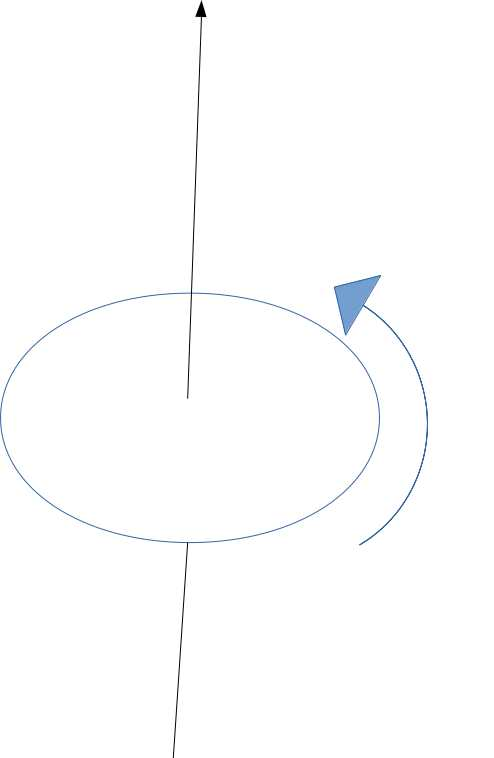
\includegraphics[width=2.0in]{campoB.jpg}
    	\label{fig:sample_figure}		
	\end{tabular}
	
\end{minipage}%

\vspace{10mm}

Secondo definizione, la velocit\'a angolare \'e
{ \Large \begin{IEEEeqnarray}{lCr}
	\omega = \frac{\Delta \alpha}{\Delta t} = \frac{v}{r}
\end{IEEEeqnarray} }

Usiamo i pedici 1 e 2 per identificare le grandezze di, rispettivamente, il primo e il secondo punto materiale


{ \Large \begin{IEEEeqnarray}{lCr}
 {\setstretch{2.25}%Distance between two following lines
\left\{ \begin{array}{ccc}
\omega_1 & = & \frac{V_1}{r} = \frac{\Delta\alpha_1}{\Delta t} \\ 
\omega_2 & = & \frac{V_2}{r} = \frac{2\pi - \Delta\alpha_1}{\Delta t}
\end{array}
\right. } \label{eq:sistema}
\end{IEEEeqnarray} }


Esplicitando $\Delta t$ nella prima delle equazioni \ref{eq:sistema} 
\begin{equation}
	\Delta t = \frac{\Delta \alpha_1 r}{V_1}
\end{equation}

E sostituendo nella seconda, si ha

\begin{eqnarray}
	\frac{V_2}{r} & = & \frac{2\pi - \Delta\alpha_1}{\Delta\alpha_1 r/V_1} \label{eq:dopo}
\end{eqnarray}

e quindi

\begin{equation}
	\frac{\Delta \alpha_1r}{V_1}\cdot\frac{V_2}{r} = 2\pi - \Delta\alpha_1
\end{equation}



\section{Introduction}

Calcolare il risultato della seguente equazione
\begin{eqnarray}
	x = 2 + 2
\end{eqnarray}

\end{document}